

%% This file was auto-generated by IPython.
%% Conversion from the original notebook file:
%%
\documentclass[11pt,english]{article}

%% This is the automatic preamble used by IPython.  Note that it does *not*
%% include a documentclass declaration, that is added at runtime to the overall
%% document.

\usepackage{amsmath}
\usepackage{amssymb}
\usepackage{graphicx}
\usepackage{grffile}
\usepackage{ucs}
\usepackage[utf8x]{inputenc}

% Scale down larger images
\usepackage[export]{adjustbox}

%fancy verbatim
\usepackage{fancyvrb}
% needed for markdown enumerations to work
\usepackage{enumerate}

% Slightly bigger margins than the latex defaults
\usepackage{geometry}
\geometry{verbose,tmargin=3cm,bmargin=3cm,lmargin=2.5cm,rmargin=2.5cm}

% Define a few colors for use in code, links and cell shading
\usepackage{color}
\definecolor{orange}{cmyk}{0,0.4,0.8,0.2}
\definecolor{darkorange}{rgb}{.71,0.21,0.01}
\definecolor{darkgreen}{rgb}{.12,.54,.11}
\definecolor{myteal}{rgb}{.26, .44, .56}
\definecolor{gray}{gray}{0.45}
\definecolor{lightgray}{gray}{.95}
\definecolor{mediumgray}{gray}{.8}
\definecolor{inputbackground}{rgb}{.95, .95, .85}
\definecolor{outputbackground}{rgb}{.95, .95, .95}
\definecolor{traceback}{rgb}{1, .95, .95}

% new ansi colors
\definecolor{brown}{rgb}{0.54,0.27,0.07}
\definecolor{purple}{rgb}{0.5,0.0,0.5}
\definecolor{darkgray}{gray}{0.25}
\definecolor{lightred}{rgb}{1.0,0.39,0.28}
\definecolor{lightgreen}{rgb}{0.48,0.99,0.0}
\definecolor{lightblue}{rgb}{0.53,0.81,0.92}
\definecolor{lightpurple}{rgb}{0.87,0.63,0.87}
\definecolor{lightcyan}{rgb}{0.5,1.0,0.83}

% Framed environments for code cells (inputs, outputs, errors, ...).  The
% various uses of \unskip (or not) at the end were fine-tuned by hand, so don't
% randomly change them unless you're sure of the effect it will have.
\usepackage{framed}

% remove extraneous vertical space in boxes
\setlength\fboxsep{0pt}

% codecell is the whole input+output set of blocks that a Code cell can
% generate.

% TODO: unfortunately, it seems that using a framed codecell environment breaks
% the ability of the frames inside of it to be broken across pages.  This
% causes at least the problem of having lots of empty space at the bottom of
% pages as new frames are moved to the next page, and if a single frame is too
% long to fit on a page, will completely stop latex from compiling the
% document.  So unless we figure out a solution to this, we'll have to instead
% leave the codecell env. as empty.  I'm keeping the original codecell
% definition here (a thin vertical bar) for reference, in case we find a
% solution to the page break issue.

%% \newenvironment{codecell}{%
%%     \def\FrameCommand{\color{mediumgray} \vrule width 1pt \hspace{5pt}}%
%%    \MakeFramed{\vspace{-0.5em}}}
%%  {\unskip\endMakeFramed}

% For now, make this a no-op...
\newenvironment{codecell}{}

 \newenvironment{codeinput}{%
   \def\FrameCommand{\colorbox{inputbackground}}%
   \MakeFramed{\advance\hsize-\width \FrameRestore}}
 {\unskip\endMakeFramed}

\newenvironment{codeoutput}{%
   \def\FrameCommand{\colorbox{outputbackground}}%
   \vspace{-1.4em}
   \MakeFramed{\advance\hsize-\width \FrameRestore}}
 {\unskip\medskip\endMakeFramed}

\newenvironment{traceback}{%
   \def\FrameCommand{\colorbox{traceback}}%
   \MakeFramed{\advance\hsize-\width \FrameRestore}}
 {\endMakeFramed}

% Use and configure listings package for nicely formatted code
\usepackage{listingsutf8}
\lstset{
  language=python,
  inputencoding=utf8x,
  extendedchars=\true,
  aboveskip=\smallskipamount,
  belowskip=\smallskipamount,
  xleftmargin=2mm,
  breaklines=true,
  basicstyle=\small \ttfamily,
  showstringspaces=false,
  keywordstyle=\color{blue}\bfseries,
  commentstyle=\color{myteal},
  stringstyle=\color{darkgreen},
  identifierstyle=\color{darkorange},
  columns=fullflexible,  % tighter character kerning, like verb
}

% The hyperref package gives us a pdf with properly built
% internal navigation ('pdf bookmarks' for the table of contents,
% internal cross-reference links, web links for URLs, etc.)
\usepackage{hyperref}
\hypersetup{
  breaklinks=true,  % so long urls are correctly broken across lines
  colorlinks=true,
  urlcolor=blue,
  linkcolor=darkorange,
  citecolor=darkgreen,
  }

% hardcode size of all verbatim environments to be a bit smaller
\makeatletter 
\g@addto@macro\@verbatim\small\topsep=0.5em\partopsep=0pt
\makeatother 

% Prevent overflowing lines due to urls and other hard-to-break entities.
\sloppy




\begin{document}


\section{{[}WS13/14{]} Mathematics for Robotics and Control Assignment
010 - Root Locus}


\begin{codecell}


\begin{codeinput}
\begin{lstlisting}
import IPython.core.display
import sys
import sympy
if not "win" in sys.platform and not "linux" in sys.platform:
    %pylab
else:
    %pylab inline
\end{lstlisting}
\end{codeinput}
\begin{codeoutput}


\begin{Verbatim}[commandchars=\\\{\}]
Populating the interactive namespace from numpy and matplotlib
\end{Verbatim}

\end{codeoutput}

\end{codecell}
\subsubsection{1. Create a new IPython notebook}


Here it is!
\subsubsection{3. Familiarize yourself with the attached rlocus2.py file
and it's functions, which you may use to work on the assignments.}


\begin{codecell}


\begin{codeinput}
\begin{lstlisting}
execfile("rlocus2.py")
#you want to use and klick: rlocusfind(G)
\end{lstlisting}
\end{codeinput}

\end{codecell}
\subsubsection{2. From the ebook linked last week (Nise), do problem
8.19, 8.22 a-c (inclusive), 8.26 a-c (inclusive) and 8.39}


\begin{codecell}


\begin{codeinput}
\begin{lstlisting}
from sympy.abc import s, K
from control import *
from math import pi
\end{lstlisting}
\end{codeinput}

\end{codecell}

\begin{codecell}


\begin{codeinput}
\begin{lstlisting}
IPython.core.display.Image("images/fig83.png", embed=True)
\end{lstlisting}
\end{codeinput}
\begin{codeoutput}



\begin{center}
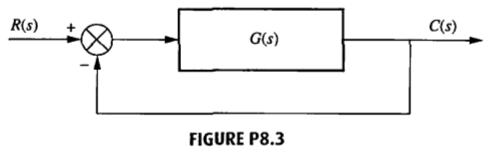
\includegraphics[max size={0.7\textwidth}{0.9\textheight}]{MRC_QUIGNONCHRISTOPHE_20140609_files/MRC_QUIGNONCHRISTOPHE_20140609_8_0.png}
\par
\end{center}


\end{codeoutput}

\end{codecell}
\paragraph{8.19}


\begin{codecell}


\begin{codeinput}
\begin{lstlisting}
IPython.core.display.Image("images/19.png", embed=True)
\end{lstlisting}
\end{codeinput}
\begin{codeoutput}



\begin{center}
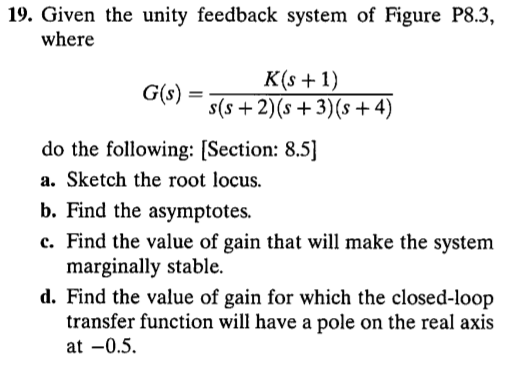
\includegraphics[max size={0.7\textwidth}{0.9\textheight}]{MRC_QUIGNONCHRISTOPHE_20140609_files/MRC_QUIGNONCHRISTOPHE_20140609_10_0.png}
\par
\end{center}


\end{codeoutput}

\end{codecell}

\begin{codecell}


\begin{codeinput}
\begin{lstlisting}
nominator = K*(s+1)
denominator = s*(s+2)*(s+3)*(s+4)
sympy.expand(denominator)
\end{lstlisting}
\end{codeinput}
\begin{codeoutput}




\begin{verbatim}
s**4 + 9*s**3 + 26*s**2 + 24*s
\end{verbatim}



\end{codeoutput}

\end{codecell}

\begin{codecell}


\begin{codeinput}
\begin{lstlisting}
#a) sketch the root locus
G = tf([1, 1], [1, 9, 26, 24, 0])
#sys = feedback(G, tf([1], [1])) #Feedback system with -1
rloc = rlocus(G)
#rlocusfind(G)
\end{lstlisting}
\end{codeinput}
\begin{codeoutput}


\begin{center}
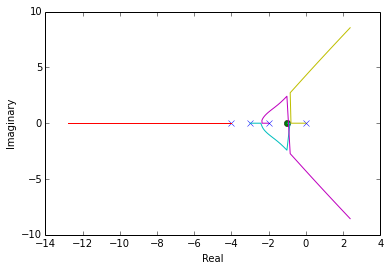
\includegraphics[max size={0.7\textwidth}{0.9\textheight}]{MRC_QUIGNONCHRISTOPHE_20140609_files/MRC_QUIGNONCHRISTOPHE_20140609_12_0.png}
\par
\end{center}

\end{codeoutput}

\end{codecell}

\begin{codecell}


\begin{codeinput}
\begin{lstlisting}
#b) Find the asymptotes (= real axis intercept, page 401)
poles, zeros = pzmap.pzmap(G)
realaxisintercept = (sum(poles)-sum(zeros))/(len(poles)-len(zeros))
print "real axis intercept: ", realaxisintercept

k = len(poles)-len(zeros)-1
angle = [((2*k_+1)*pi)/(len(poles)-len(zeros)) for k_ in arange(0, k)]
print "angles: ", angle
\end{lstlisting}
\end{codeinput}
\begin{codeoutput}


\begin{Verbatim}[commandchars=\\\{\}]
real axis intercept:  -2.66666666667
angles:  [1.0471975511965976, 3.1415926535897931]
\end{Verbatim}

\begin{center}
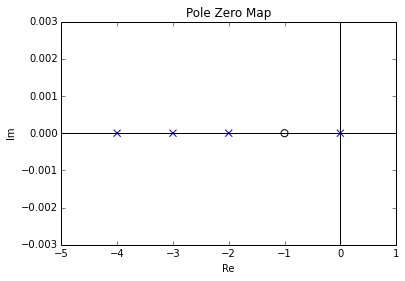
\includegraphics[max size={0.7\textwidth}{0.9\textheight}]{MRC_QUIGNONCHRISTOPHE_20140609_files/MRC_QUIGNONCHRISTOPHE_20140609_13_1.png}
\par
\end{center}

\end{codeoutput}

\end{codecell}

\begin{codecell}


\begin{codeinput}
\begin{lstlisting}
#c) marginable stable

#The system is marginally stable where the root locus crosses the imaginary axis
#gain at the imaginary axis = K = ~140
rloc = rlocus(G)
\end{lstlisting}
\end{codeinput}
\begin{codeoutput}


\begin{center}
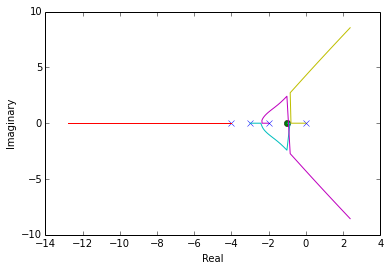
\includegraphics[max size={0.7\textwidth}{0.9\textheight}]{MRC_QUIGNONCHRISTOPHE_20140609_files/MRC_QUIGNONCHRISTOPHE_20140609_14_0.png}
\par
\end{center}

\end{codeoutput}

\end{codecell}

\begin{codecell}


\begin{codeinput}
\begin{lstlisting}
#d) Find the Value of gain for which the closed-loop transfer funcion will have a pole on the real axis at -0.5
#rlocusfind(G) at -0.5 on the real axis
#Gain ~13
\end{lstlisting}
\end{codeinput}

\end{codecell}
\paragraph{8.22 a-c}


\begin{codecell}


\begin{codeinput}
\begin{lstlisting}
IPython.core.display.Image("images/22.png", embed=True)
\end{lstlisting}
\end{codeinput}
\begin{codeoutput}



\begin{center}
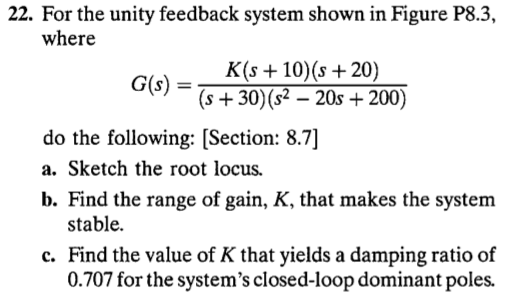
\includegraphics[max size={0.7\textwidth}{0.9\textheight}]{MRC_QUIGNONCHRISTOPHE_20140609_files/MRC_QUIGNONCHRISTOPHE_20140609_17_0.png}
\par
\end{center}


\end{codeoutput}

\end{codecell}

\begin{codecell}


\begin{codeinput}
\begin{lstlisting}
nominator = K*(s+10)*(s+20)
denominator = (s+30)*(s**2-20*s+200)
print sympy.expand(nominator)
print sympy.expand(denominator)
\end{lstlisting}
\end{codeinput}
\begin{codeoutput}


\begin{Verbatim}[commandchars=\\\{\}]
K*s**2 + 30*K*s + 200*K
s**3 + 10*s**2 - 400*s + 6000
\end{Verbatim}

\end{codeoutput}

\end{codecell}

\begin{codecell}


\begin{codeinput}
\begin{lstlisting}
# a) sketch the root locus
g = (tf([1, 30, 200],[1, 10, -400, 6000]))
rloc = rlocus(g)
\end{lstlisting}
\end{codeinput}
\begin{codeoutput}


\begin{center}
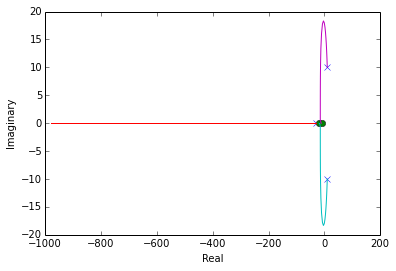
\includegraphics[max size={0.7\textwidth}{0.9\textheight}]{MRC_QUIGNONCHRISTOPHE_20140609_files/MRC_QUIGNONCHRISTOPHE_20140609_19_0.png}
\par
\end{center}

\end{codeoutput}

\end{codecell}

\begin{codecell}


\begin{codeinput}
\begin{lstlisting}
# b) find the range of gain, K, that makes the system stable
#The lowest gain is the gai where the tf crosses the real axis: ~24
#The highest gain is it at the pole of -11 where the gain is ~1200
#The instable part to the right side has gain lower then 24
\end{lstlisting}
\end{codeinput}

\end{codecell}

\begin{codecell}


\begin{codeinput}
\begin{lstlisting}
# c) find the value of K that yields a damping ratio of .707 for the systems closed-loop dominant poles
# The damping ratio can be found at ~(-13.7, 11.35) and the gain there is ~80
\end{lstlisting}
\end{codeinput}

\end{codecell}
\paragraph{8.26 a-c}


\begin{codecell}


\begin{codeinput}
\begin{lstlisting}
IPython.core.display.Image("images/26_1.png", embed=True)
\end{lstlisting}
\end{codeinput}
\begin{codeoutput}



\begin{center}
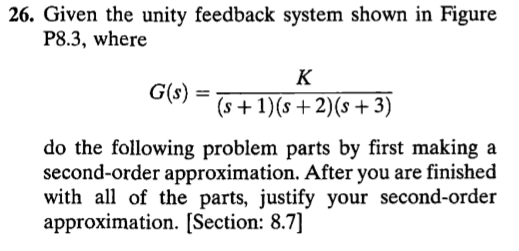
\includegraphics[max size={0.7\textwidth}{0.9\textheight}]{MRC_QUIGNONCHRISTOPHE_20140609_files/MRC_QUIGNONCHRISTOPHE_20140609_23_0.png}
\par
\end{center}


\end{codeoutput}

\end{codecell}

\begin{codecell}


\begin{codeinput}
\begin{lstlisting}
IPython.core.display.Image("images/26_2.png", embed=True)
\end{lstlisting}
\end{codeinput}
\begin{codeoutput}



\begin{center}
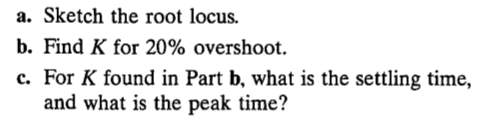
\includegraphics[max size={0.7\textwidth}{0.9\textheight}]{MRC_QUIGNONCHRISTOPHE_20140609_files/MRC_QUIGNONCHRISTOPHE_20140609_24_0.png}
\par
\end{center}


\end{codeoutput}

\end{codecell}

\begin{codecell}


\begin{codeinput}
\begin{lstlisting}
denominator = (s+1)*(s+2)*(s+3)
sympy.expand(denominator)
\end{lstlisting}
\end{codeinput}
\begin{codeoutput}




\begin{verbatim}
s**3 + 6*s**2 + 11*s + 6
\end{verbatim}



\end{codeoutput}

\end{codecell}

\begin{codecell}


\begin{codeinput}
\begin{lstlisting}
# a) sketch the root locus
g = (tf([1],[1, 6, 11, 6]))
rloc = rlocus(g)
\end{lstlisting}
\end{codeinput}

\end{codecell}

\begin{codecell}


\begin{codeinput}
\begin{lstlisting}
# b) find K for 20% overshoot
#The 20% overshoot can be found at Pole: ~(-8.60, +16.90)
#Gain 9.14369084667
#Pole: (-0.880170395421+1.67521158854j)

\end{lstlisting}
\end{codeinput}

\end{codecell}

\begin{codecell}


\begin{codeinput}
\begin{lstlisting}
# c) For K found in b) what is the settling time, what is the peak time?
g = (tf([1],[1, 6, 11, 6+9]))
#6+K because of charcteristic equation 1+KG(s)=0
step = step_response(g)
plot(step[0], step[1])
#peak time is ~2.1
#settling time ~5
\end{lstlisting}
\end{codeinput}
\begin{codeoutput}




\begin{verbatim}
[<matplotlib.lines.Line2D at 0x5af6810>]
\end{verbatim}



\begin{center}
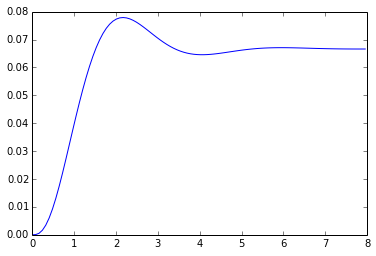
\includegraphics[max size={0.7\textwidth}{0.9\textheight}]{MRC_QUIGNONCHRISTOPHE_20140609_files/MRC_QUIGNONCHRISTOPHE_20140609_28_1.png}
\par
\end{center}

\end{codeoutput}

\end{codecell}
\paragraph{8.39}


\begin{codecell}


\begin{codeinput}
\begin{lstlisting}
IPython.core.display.Image("images/39.png", embed=True)
\end{lstlisting}
\end{codeinput}
\begin{codeoutput}



\begin{center}
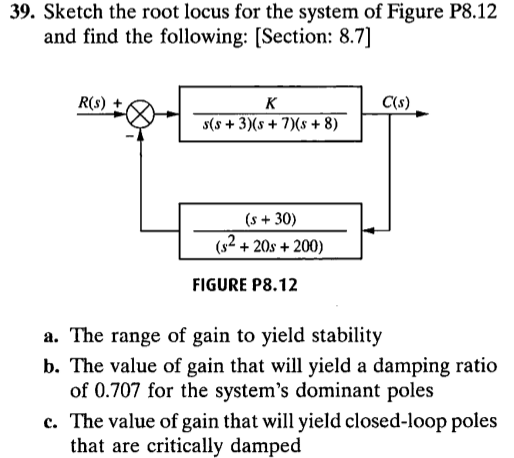
\includegraphics[max size={0.7\textwidth}{0.9\textheight}]{MRC_QUIGNONCHRISTOPHE_20140609_files/MRC_QUIGNONCHRISTOPHE_20140609_30_0.png}
\par
\end{center}


\end{codeoutput}

\end{codecell}

\begin{codecell}


\begin{codeinput}
\begin{lstlisting}
denominator = s*(s+3)*(s+7)*(s+8)
sympy.expand(denominator)
\end{lstlisting}
\end{codeinput}
\begin{codeoutput}




\begin{verbatim}
s**4 + 18*s**3 + 101*s**2 + 168*s
\end{verbatim}



\end{codeoutput}

\end{codecell}

\begin{codecell}


\begin{codeinput}
\begin{lstlisting}
upper = tf([1], [1, 18, 101, 168, 0])
lower = tf([1, 30], [1, 20, 200])

g = feedback(upper, lower)
rloc = rlocus(g)
\end{lstlisting}
\end{codeinput}
\begin{codeoutput}


\begin{center}
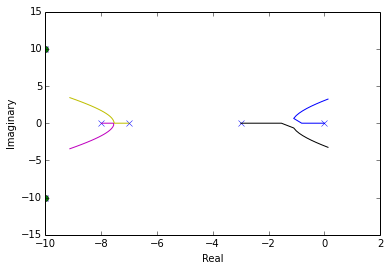
\includegraphics[max size={0.7\textwidth}{0.9\textheight}]{MRC_QUIGNONCHRISTOPHE_20140609_files/MRC_QUIGNONCHRISTOPHE_20140609_32_0.png}
\par
\end{center}

\end{codeoutput}

\end{codecell}

\begin{codecell}


\begin{codeinput}
\begin{lstlisting}
# a) The range of gain to yield stability
#In the stable range the gain goes from 0 to 1000
#In the unstable range it goes from 850 to 1000
#Thus we can not certainly conclude stability from gain
\end{lstlisting}
\end{codeinput}

\end{codecell}

\begin{codecell}


\begin{codeinput}
\begin{lstlisting}
# b) The value of gain that will yield a damping ratio of 0.707 for the systems dominant poles
#Gain: 137
#Pole: (-1.00, 1.01)
\end{lstlisting}
\end{codeinput}

\end{codecell}

\begin{codecell}


\begin{codeinput}
\begin{lstlisting}
# c) The value of gain that will yield closed-loop poles that are critically damped
# The system is critically damped where damping factor is 1.
# The value of gain: 3.41 at Pole: (-7.89, +0)
\end{lstlisting}
\end{codeinput}

\end{codecell}
\subsubsection{4. Submit your solutions in your newly created IPython
file}


Here it is.



\end{document}

